\problem{}
Execute the Ford-Fulkerson algorithm on the flow network shown in the figure below. Display the residual network after each flow update and determine the maximum flow at the end. During each iteration, choose the lexicographically smallest available augmenting path. For example, if two augmenting paths are \(s \to 2 \to t\) and \(s \to 3 \to t\), select \(s \to 2 \to t\) since it is lexicographically smaller. Likewise, if the paths \(s \to 3 \to t\) and \(s \to 2 \to 4 \to t\) are available, choose \(s \to 2 \to 4 \to t\).
\begin{figure}[h]
    \centering
    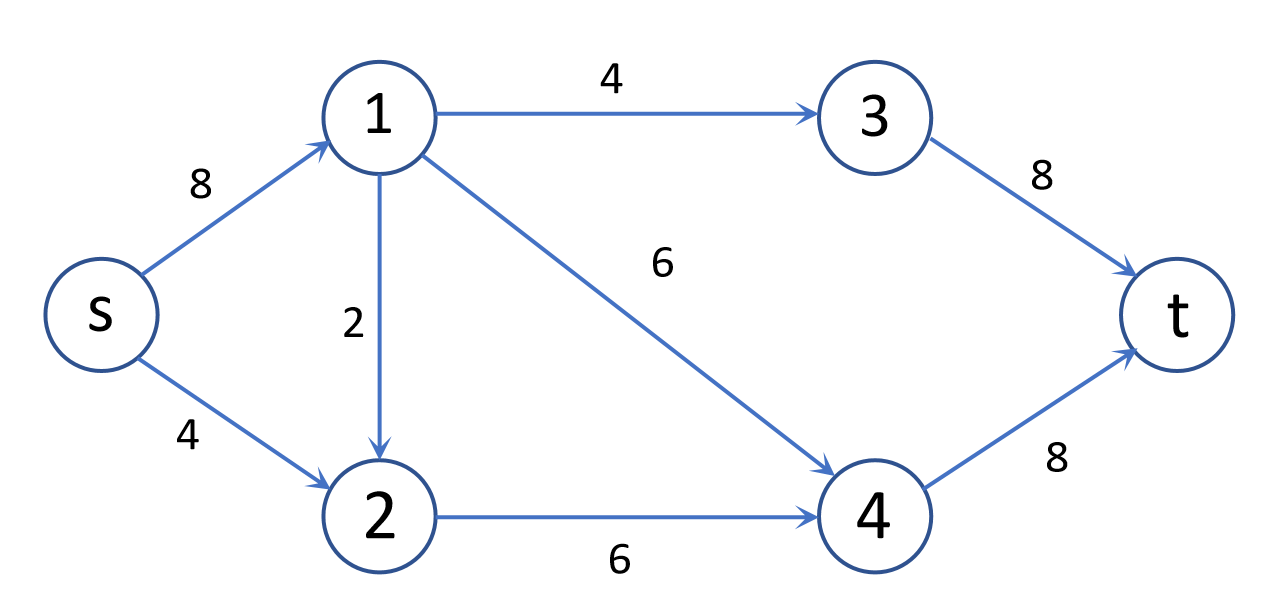
\includegraphics[width=0.75\linewidth]{HW2.png}
\end{figure}

\solution{
}

\newpage